\documentclass[12pt]{article}
\usepackage{./common/karnaugh-map}
\usepackage{scrextend}
\usepackage[utf8]{inputenc}
\usepackage[polish]{babel}
\usepackage[T1]{fontenc}%polskie znaki
\usepackage[utf8]{inputenc}%polskie znaki
\usepackage{geometry}
\usepackage{float}
\usepackage{enumitem}
\usepackage{hyperref}
\usepackage{graphicx}
\usepackage{tabulary}
\usepackage{etoc}
\usepackage[normalem]{ulem} 
\renewcommand{\baselinestretch}{1.5}
\graphicspath{ {img/} }
\newgeometry{lmargin=2.5cm, rmargin=2.5cm, tmargin=2.5cm, bmargin=2.5cm}
\usepackage{tikz}
\usepackage[bf]{caption}
\usepackage{subcaption}
\usepackage{amsmath}
\usepackage{listings}
\usepackage{tikz}

\usepackage{tikz-timing}
\definecolor{codegreen}{rgb}{0,0.6,0}
\definecolor{codegray}{rgb}{0.5,0.5,0.5}
\definecolor{codepurple}{rgb}{0.58,0,0.82}
\definecolor{backcolour}{rgb}{0.95,0.95,0.93}
 
\lstdefinestyle{mystyle}{
    backgroundcolor=\color{backcolour},   
    commentstyle=\color{codegreen},
    keywordstyle=\color{magenta},
    numberstyle=\tiny\color{codegray},
    stringstyle=\color{codepurple},
    basicstyle=\ttfamily\footnotesize,
    breakatwhitespace=false,         
    captionpos=b,                    
    keepspaces=true,                 
    numbers=left,                    
    numbersep=5pt,                  
    showspaces=false,                
    showstringspaces=false,
    showtabs=false,                  
    tabsize=2,
    breaklines=true,
    postbreak=\mbox{\textcolor{red}{$\hookrightarrow$}\space},
}
\lstset{style=mystyle}

\title{ 
    \vspace*{50mm}
    \textsc{
        \textbf{Układy Cyfrowe i Systemy Wbudowane 2}\\
        \large Projekt \\
         Organy z pozytywką
    }
} 
\author{
Maja Bojarska, 241287\\
Damian Koper,  241292\\
}

\date{\today}

\begin{document}

\maketitle

\newpage

\section{Cel projektu}

Celem projektu było wykonanie układu realizującego działanie organów, sterowanych za pomocą klawiszy klawiatury, podłączonej poprzez interfejs PS2. Rozszerzeniem działania układu było odtwarzanie sekwencji dźwięków odczytanej z pliku tekstowego, zapisanego na karcie pamięci typu SD.

\subsection{Założenia wstępne}

Początkowy projekt układu zakładał podział kolejnych funkcjonalności na możliwie małe moduły, według zasady pojedynczej odpowiedzialności. Układ mapował klawisze klawiatury na odpowiadające im dźwięki. Klawisze były przypisane do dźwięków, zgodnie z układem przybliżonym do klawiszy jednej oktawy pianina.  Oktawa zmieniana była za pomocą klawiszy strzałek w zakresie od 0 do 8.

\begin{figure}[h]
  \centering
  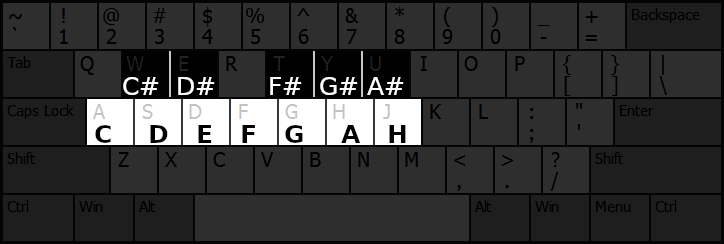
\includegraphics[width=\linewidth]{images/key_mapping.png}
  \caption{Przypisanie tonów oktawy do klawiszy klawiatury QWERTY. Poniżej każdej litery klawisza znajduje się odpowiadający mu ton.}
  \label{kay_mapping}
\end{figure}

Pierwotny projekt zakładał również podział na wiele rodzajów fal. Rodzaj fali miał być wybierany poprzez obracanie enkodera cyfrowego w lewo (poprzedni) lub prawo (następny). Diagram przepływu danych wstępnej wersji projektu, został przedstawiony na rysunku \ref{base}.

\begin{figure}[h]
  \centering
  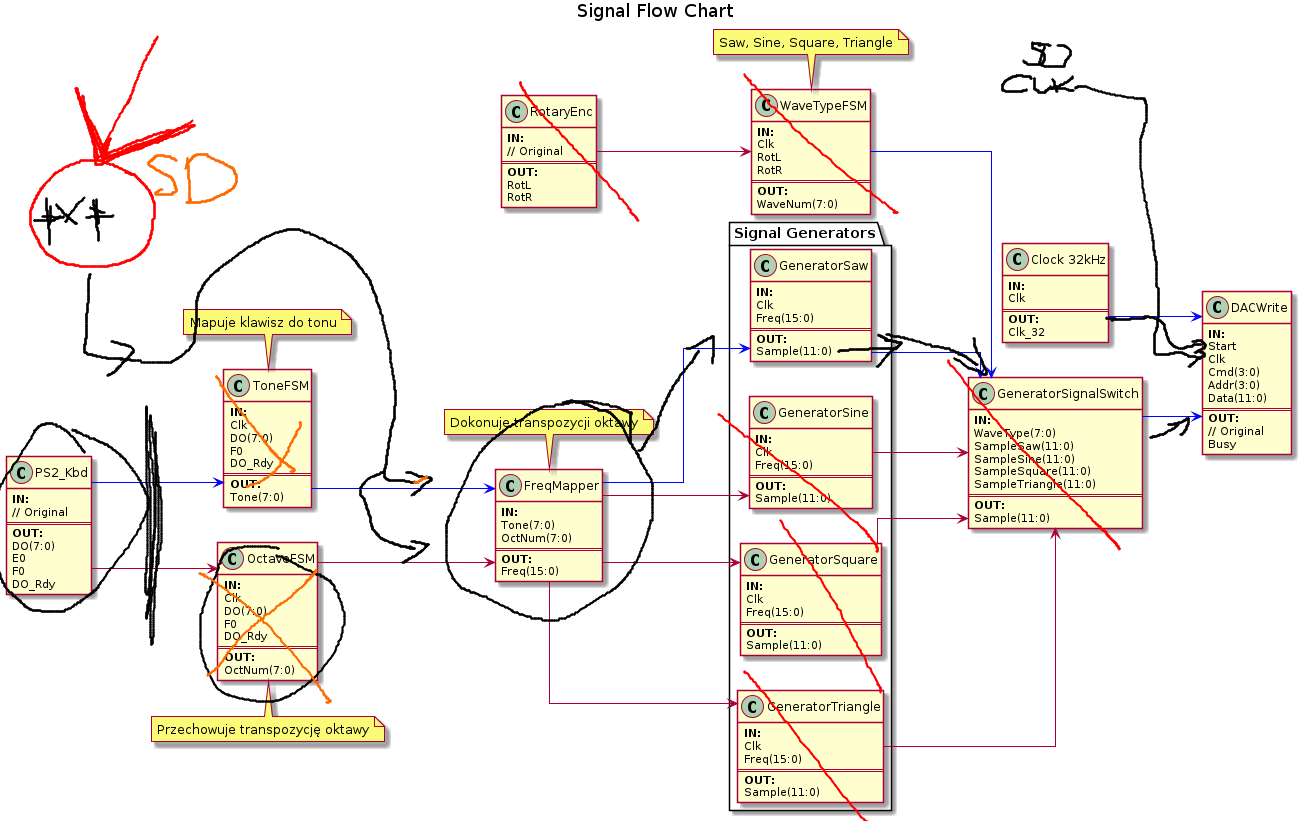
\includegraphics[width=\linewidth]{./diagram/out/flow_chart}
  \caption{Wstępny projekt organów. Niebieskimi strzałkami oznaczono podstawową i~wykonaną jako pierwszą funkcjonalność. }
  \label{base}
\end{figure}

\subsection{Założenia rozszerzone}

Rozszerzeniem funkcjonalności organów sterowanych za pomocą klawiatury było uzyskanie możliwości odtwarzania wcześniej zapisanej sekwencji dźwięków o~zmiennej długości. Wykorzystano do tego możliwość wczytania danych z karty pamięci i moduł \textit{SDC\_FileReader}.
Przykład zapisu dźwięku w pliku tekstowym:
\begin{align*}
  a401
\end{align*}
gdzie:
\begin{align*}
  a                & - Klawisz\;na\;klawiaturze\;QWERTY \\
  4                & - Oktawa                           \\
  01 & - Czas\;trwania\;[x*10ms]           \\
\end{align*}
Jeden dźwięk jest zawsze definiowany z wykorzystaniem 4 znaków, więc zapis nie wymaga stosowania separatorów. Czas trwania dźwięku zapisany jest z wykorzystaniem liczby dziesiętnej zapisanej tekstowo na 2 znakach. Definiuje ona czas trwania dźwięku, jako wielokrotność $10ms$.

\section{Struktura układu}
\subsection{Schemat najwyższego poziomu}
Schemat najwyższego poziomu, przedstawiony na rysunku \ref{sch:main}, zawiera wszystkie zewnętrzne moduły odpowiedzialne za komunikację z urządzeniami peryferyjnymi. Są to:
\begin{itemize}[noitemsep]
  \item \textit{SDC\_FileReader}
  \item \textit{PS2\_Kbd}
  \item \textit{DACWrite}
\end{itemize}
Wszystkie moduły komunikują się z modułem \textit{InnerLogic}.


\begin{figure}[h]
  \centering
  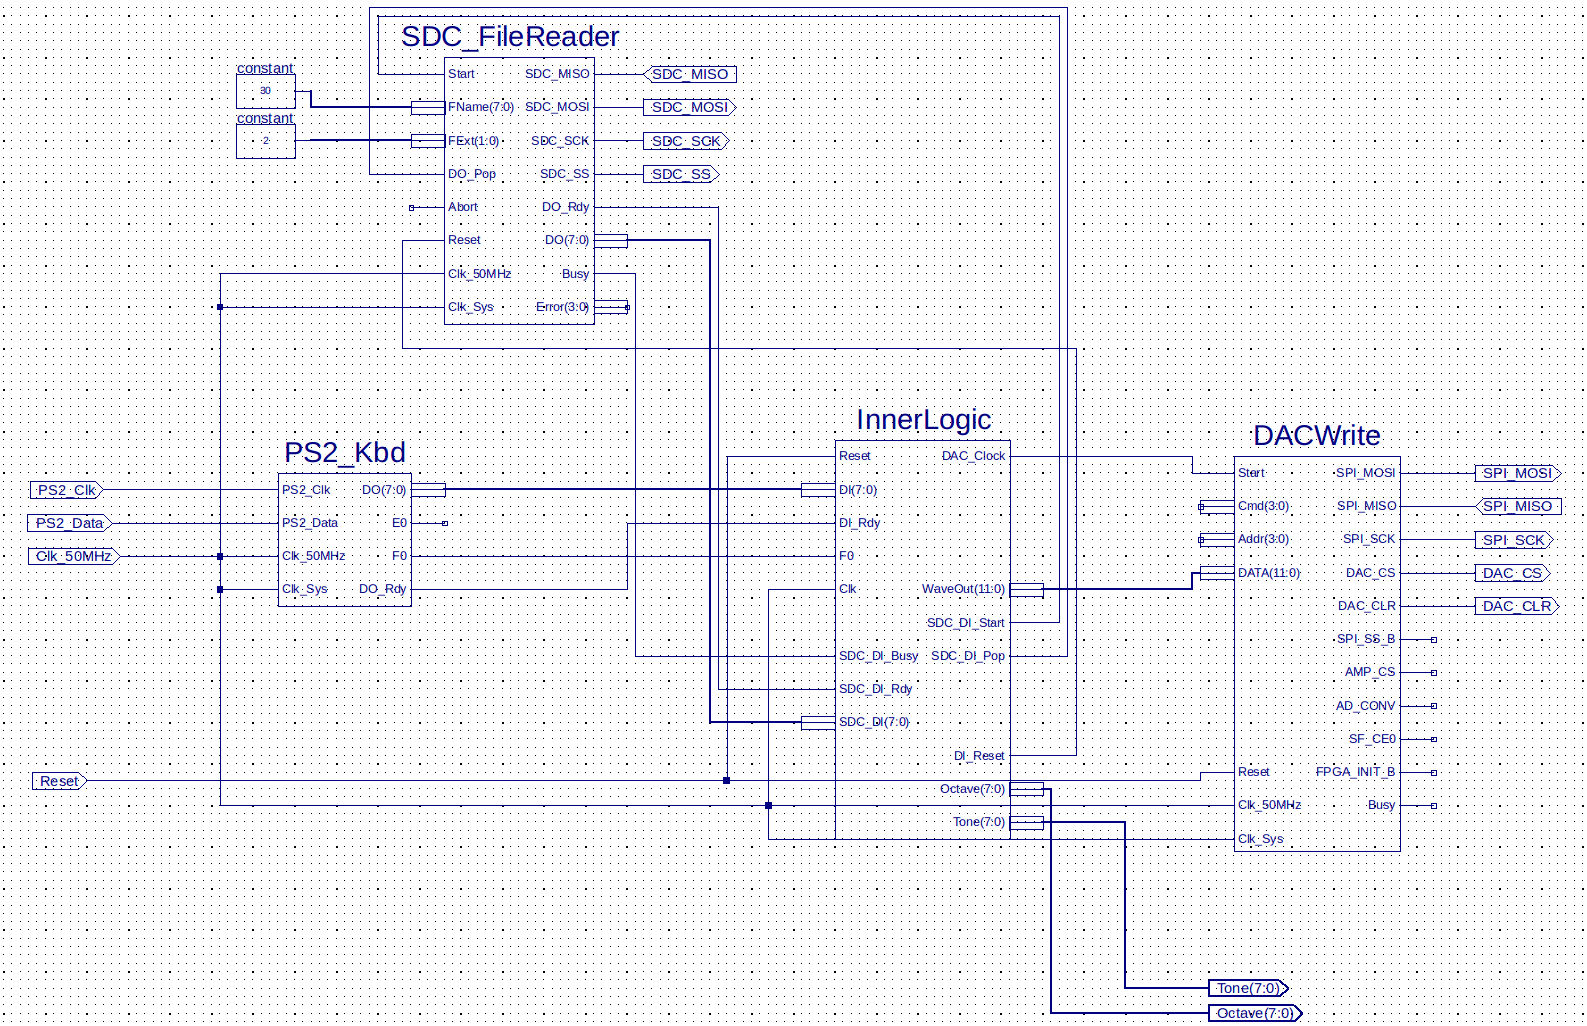
\includegraphics[width=\linewidth]{images/main}
  \caption{Schemat najwyższego poziomu.}
  \label{sch:main}
\end{figure}

\subsection{InnerLogic}

Schemat InnerLogic, przedstawiony na rysunku \ref{sch:inner}, zawiera wszystkie moduły odpowiedzialne za generowanie sygnału wyjściowego, na podstawie danych wejściowych zebranych z klawiatury i karty SD. Przedstawione tutaj moduły mają swoje częściowe odwzorowanie we wstępnym projekcie, przedstawionym na rysunku \ref{base}.

\begin{figure}[h]
  \centering
  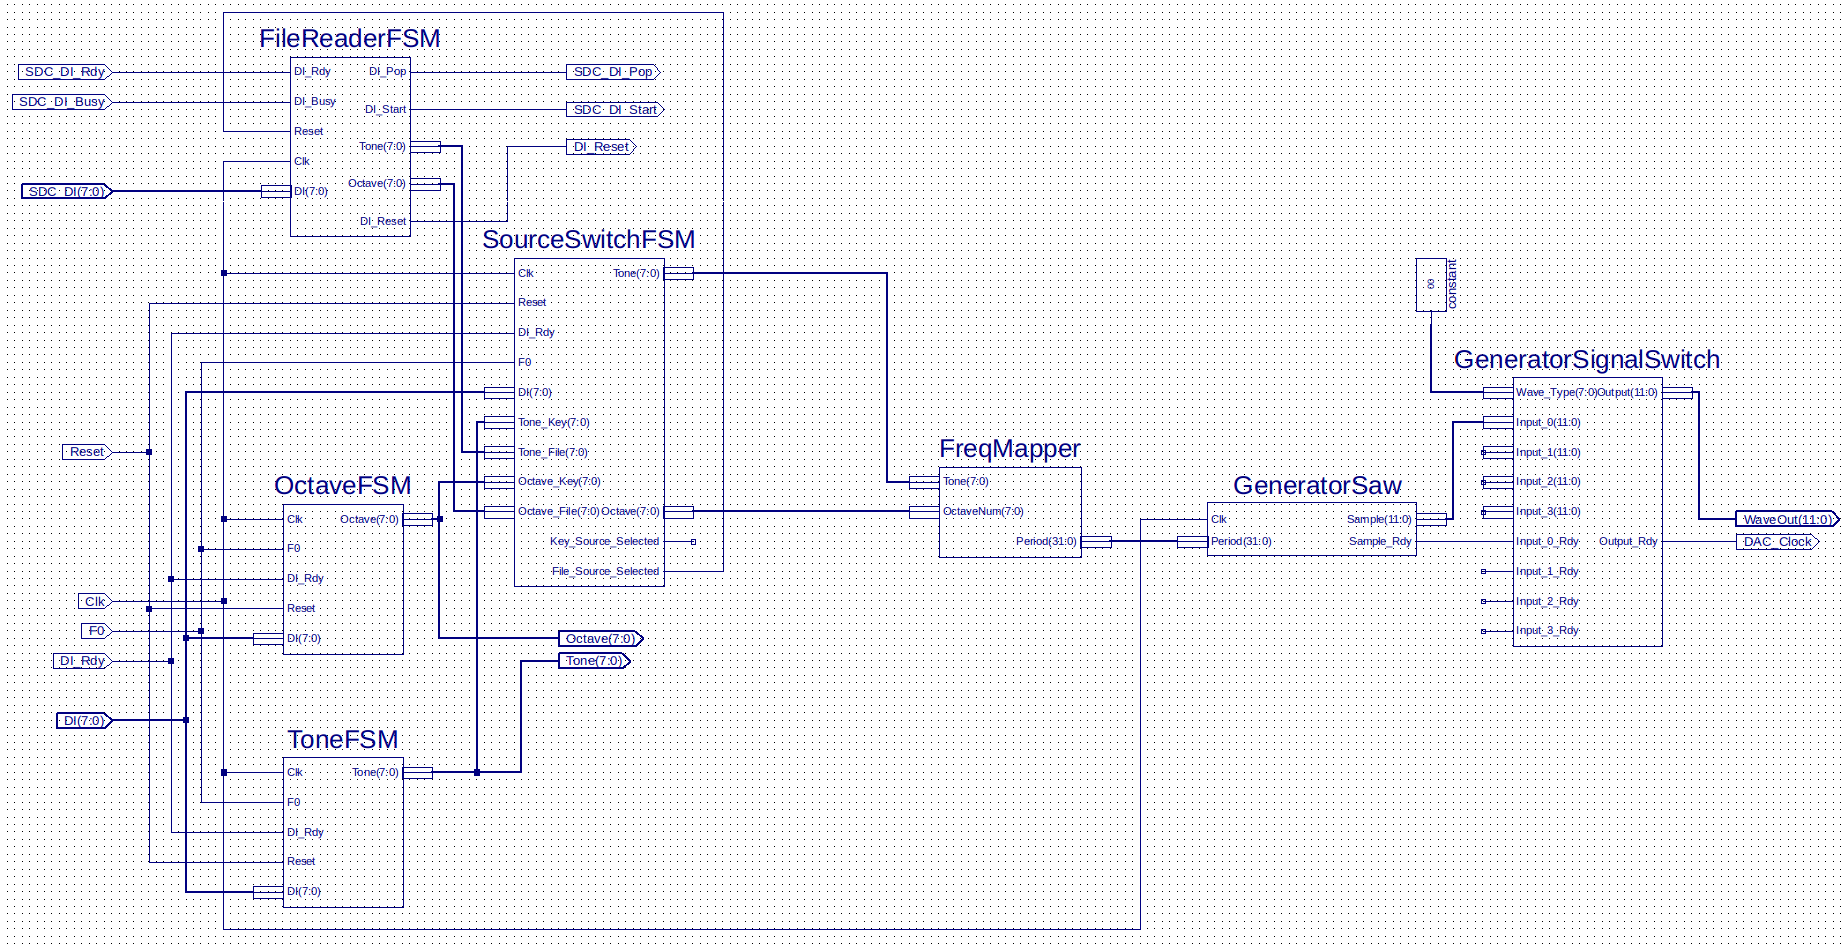
\includegraphics[width=\linewidth]{images/inner}
  \caption{Schemat InnerLogic.}
  \label{sch:inner}
\end{figure}

W celach debugowania jednymi z wyjść modułu InnerLogic są numery aktualnie odtwarzanego tonu oraz oktawy. Zostały one podłączone do diod LED układu, gdzie pierwsze cztery (7-4) pokazują zakodowany binarnie numer tonu, a ostatnie trzy (2-0) kod oktawy. 

\subsection{FileReaderFSM}

Moduł FileReaderFSM realizuje maszynę stanów, która jest odpowiedzialna za interakcjem z modułem \textit{SDC\_FileReader}. Odpowiada on za dostarczanie numeru tonu i oktawy przez określony czas, gdzie wszystkie te dane odczytywane są z karty SD.

Moduł \textit{SDC\_FileReader} umożliwia odczyt wartości z pliku podobnie do kolejki FIFO. Moduł \textit{FileReaderFSM} w procesie odczytu danych jednego dźwięku najpierw odczytuje znak tonu, potem oktawy, a następnie czas jego trwania, wpisując tę wartość do licznika. Po zakończonym odczycie 4 znaków, licznik jest uruchamiany, a wartości zmapowanych kodów tonu i oktawy są obecne na wyjściach modułu, dopóki licznik się nie wyzeruje. Wczytanie tonu $1$ i oktawy $4$ przedstawia symulacja na rysunku \ref{sim:fileReader}.

Ton i oktawa podawane są na wyjście zaraz po ich odczytaniu, a licznik uruchamiany jest po wczytaniu całego słowa określającego długość dźwięku. Skutkuje to pomijalnie małym wydłużeniem czasu trwania dźwięku.
\subsubsection{Symulacja}
\begin{figure}[h]
  \centering
  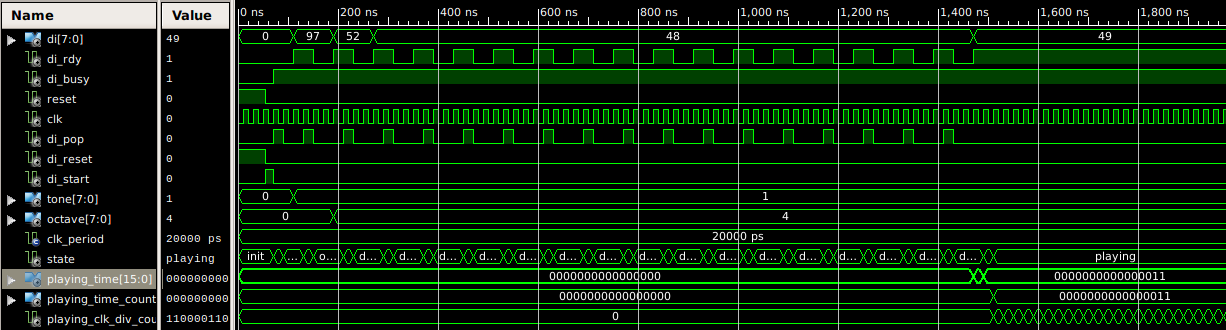
\includegraphics[decodearray={1 0 1 0 1 0}, width=\linewidth]{images/filereader}
  \caption{Symulacja modułu FileReaderFSM.}
  \label{sim:fileReader}
\end{figure}

Na rysunku \ref{sim:fileReader} w chwili $t=55ns$ widzimy zwolnienie sygnału reset i podanie sygnału start do modułu \textit{SDC\_FileReader}. Następnie moduł przechodzi przez stany na zmianę \textit{<subject>\_Request} i \textit{<subject>\_Reading}, w których kolejno popycha kolejkę odczytu z karty pamięci i zapisuje dane dostarczone przez sygnał \textit{DI}. Na końcu, w chwili $t=380ns$ moduł przechodzi do procesu dekrementowania licznika, który odlicza czas trwania dźwięku.


\subsection{ToneFSM}
ToneFSM realizuje maszynę stanów, której stan określa aktualnie odtwarzany ton.
Kody od 1 do 12 odpowiadają wszystkim tonom jednej oktawy. Kod 0 odpowiada ciszy, czyli stanowi, kiedy żaden przycisk nie jest wciśnięty. Stan maszyny zmieniany jest w momencie naciśnięcia lub puszczenia przycisku na klawiaturze i stan ten jest następnie mapowany na odpowiedni kod tonu. Kolejne wciśnięcia przycisków (A, W, S, E, D, R, F) przedstawia symulacja na rysunku \ref{sim:tone}. Kod lewej strzałki to \textit{X"1d"}, natomiast prawej \textit{X"2d"}. Warto również zauważyć, że po wciśnięciu innego klawisza nie jest zmieniany stan.

\begin{figure}[h]
  \centering
  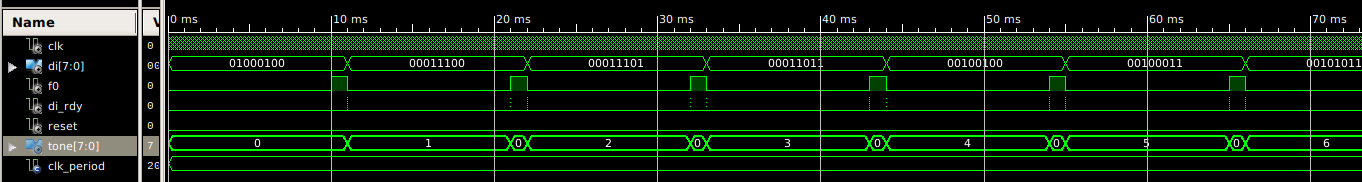
\includegraphics[decodearray={1 0 1 0 1 0}, width=\linewidth]{images/tone}
  \caption{Symulacja modułu ToneFSM.}
  \label{sim:tone}
\end{figure}


\subsection{OctaveFSM}

OctaveFSM realizuje maszynę stanów, której stan określa aktualną oktawę, względem której określane są okresy fali, dla aktualnego tonu (przez ton rozumiane są tutaj wartości całkowite, z przedziału 0-12). Stan maszyny zmieniany jest w momencie naciśnięcia strzałki lewej ($\leftarrow$) lub prawej ($\rightarrow$). Strzałka lewa zmniejsza numer oktawy o jeden, a strzałka prawa podwyższa o jeden. Zakres wartości wyjścia \textit{OctaveNum} ograniczony jest do przedziału 0-8, co odpowiada oktawom 1-9 lub inaczej, dźwiękom C1-H9. Reakcję modułu na wciśnięcia przycisków przedstawia rysunek \ref{sim:octavefsm}

\begin{figure}[h]
  \centering
  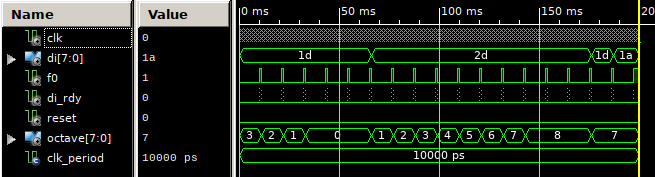
\includegraphics[decodearray={1 0 1 0 1 0}, width=\linewidth]{images/octavefsm.png}
  \caption{Symulacja modułu OctaveFSM.}
  \label{sim:octavefsm}
\end{figure}


\subsection{SourceSwitchFSM}
Moduł SourceSwitchFSM odpowiedzialny jest za wybór źródła dźwięku i za restartowanie odczytu dźwięków z karty pamięci w przypadku wyboru tego źródła. Klawisz M zmienia źródło na klawiaturę, a klawisz N na kartę pamięci. Na symulacji z rysunku \ref{sim:source} w chwili $t=320ns$ widać zmianę domyślnego źródła klawiatury na kartę pamięci i wysłanie impulsu wystąpienia zdarzenia zmiany źródła. Zdarzenie to obsługiwane jest przez moduł \textit{FileReaderFSM}, który restartuje proces odczytu.
\begin{figure}[h]
  \centering
  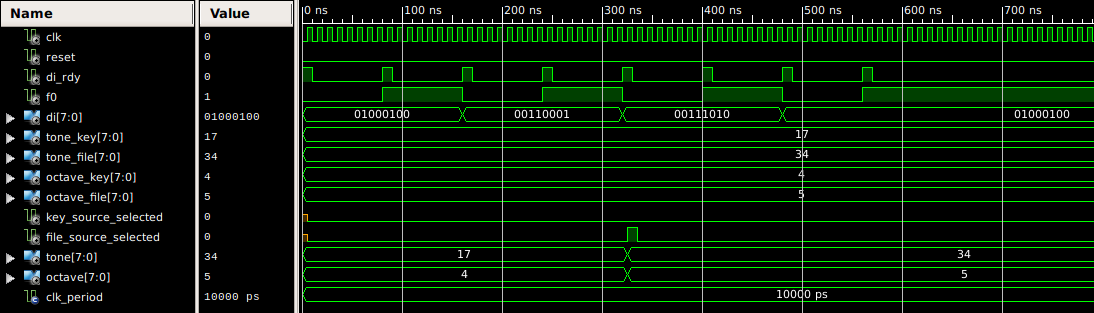
\includegraphics[decodearray={1 0 1 0 1 0}, width=\linewidth]{images/source}
  \caption{Symulacja modułu SourceSwitchFSM.}
  \label{sim:source}
\end{figure}

Działanie omawianego modułu zrealizowane jest za pomocą trzech procesów. Proces SYNC\_PROC odpowiada za przejścia pomiędzy stanami maszyny stanów oraz za wysyłanie jednotaktowych impulsów informujących o zmiania stanu. Proces NEXT\_STATE\_DECODE odpowiada za dekodowanie następnego stanu na podstawie wciśniętego klawisza, a proces OUTPUT\_ENCODE steruje sygnałami wyjściowymi przekierowyjąc odpowiednie źródło w zależności od stanu. Opis architektury przedstawia listing \ref{lst:SourceSwitchFSM}.


\subsection{FreqMapper}
FreqMapper obsługuje proces mapowania oktawy i tonu na liczbę cykli zegara o częstotliwości 50MHz, która odpowiada okresowi fali danego dźwięku. Ton 0 mapowany jest zawsze na wartość 0, co w dalszym procesie generowania sygnału oznacza ciszę. Symulację dla oktawy 0 oraz 3 przedstawia rysunek \ref{sim:mapper}. Sam proces mapowania opisuje kod z listingu \ref{lst:freqMapper} i sprowadza się on do odczytania wartości z dwuwymiarowej tablicy \lstinline{Cycles_Per_Wave_Period_Table}.
\begin{figure}[h]
  \centering
  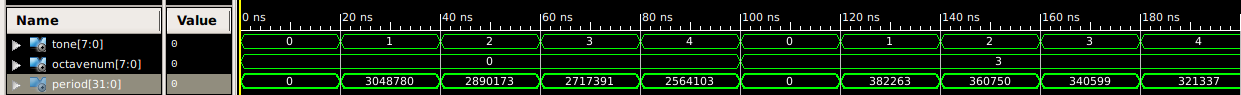
\includegraphics[decodearray={1 0 1 0 1 0}, width=\linewidth]{images/mapper}
  \caption{Symulacja modułu FreqMapper.}
  \label{sim:mapper}
\end{figure}

Zależności pomiędzy liczbą okresów $P_{C3}$, a okresem oraz częstotliwością tonu C3, opisują poniższe równania.

\[ f_{clk} = 50MHz \]
\[ T_{clk} = \frac{1}{50MHz} = 20ns \]
\[ P_{C3} = 382263 \]
\[ T_{C3} = P_{C3} * T_{clk} = 7645260ns \]
\[ f_{C3} = \frac{1}{T_{C3}} \approx 130.81Hz \]




\subsection{GeneratorSaw}

Moduł \textit{GeneratorSaw} generuje falę piłokształtną dla zadanego okresu dostarczonego z modułu \textit{FreqMapper}. Skuteczna rozdzielczość generatora wynosi 8 bitów, jednak próbki na wyjściu są przesuwane o 4 bity w lewo, aby osiągnąć zgodność z rozmiarem próbki na wejściu modułu \textit{DACWrite}.

Kolejne próbki fali generowane są w oparciu o dwa liczniki. Jeden niskiej częstotliwości (\textit{low-freq}), który odpowiada za bity 0-3, oraz drugi, o okresie 16-krotnie krótszym (\textit{high-freq}), który odpowiada za bity 4-7 próbki wynikowej. Bity 8-11 pozostają zawsze wyzerowane. Zastosowanie dwóch liczników ma na celu osiągnięcie wyższej rozdzielczości generatora, przy zachowaniu niewielkiego błędu okresu fali, który wynika z niedokładności dzielenia. Licznik \textit{high-freq} podlega pod licznik \textit{low-freq}, tzn. wyzerowanie licznika \textit{low-freq} skutkuje wyzerowaniem licznika \textit{high-freq} oraz bitów 4-7. Dzięki temu błąd czasu trwania okresu fali zostaje zredukowany.

Symulację dla modułu GeneratorSaw przedstawia rysunek \ref{sim:gen_saw}. Na wejście \textit{Period} podano następujące wartości:
\begin{equation}
  0 (cisza) \rightarrow 382263 (C3) \rightarrow 191131 (C4) \rightarrow 95547 (C5) \rightarrow 0 (cisza).
\end{equation}

Dla każdej z powyższych wartości była generowana fala w symulacji przez 20ms, z odstępami ciszy trwającymi 1ms.

\begin{figure}[h]
  \centering
  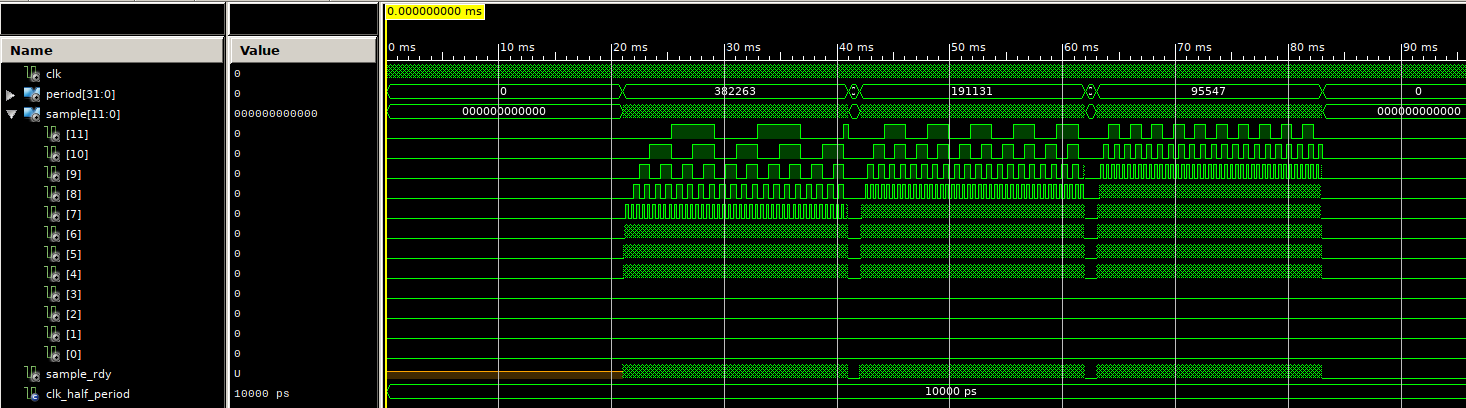
\includegraphics[decodearray={1 0 1 0 1 0}, width=\linewidth]{images/generator_saw.png}
  \caption{Symulacja modułu GeneratorSaw.}
  \label{sim:gen_saw}
\end{figure}


\subsection{GeneratorSignalSwitch}

Moduł GeneratorSignalSwitch jest multiplekserem sygnałów przychodzących z różnych generatorów fali. Rodzaj fali przekazywanej na wyjście określany jest sygnałem \textit{wave\_type}. Moduł ten przekazuje zarówno próbkę na wyjściu generatora, jak i impuls \textit{sample\_rdy}, generowany przy każdej zmianie wartości próbki. Wybór rodzaju fali X, gdzie X jest liczbą z przedziału 0-3, powoduje następujące zależności:
\[output <= input\_X\]
\[output\_rdy <= input\_X\_rdy\]

\begin{figure}[h]
  \centering
  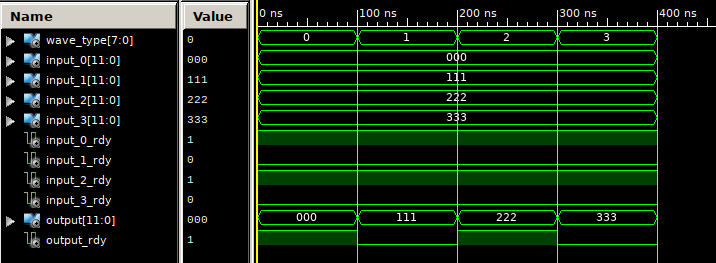
\includegraphics[decodearray={1 0 1 0 1 0}, width=\linewidth]{images/generator_signal_switch.png}
  \caption{Symulacja modułu GeneratorSignalSwitch.}
  \label{sim:gen_signal_switch}
\end{figure}


\section{Symulacja InnerLogic}
Oba warianty wejść zostały odpowiednio przetestowane w symulacji. Rysuneki \ref{sim:kb} i \ref{sim:sd} przedstawiają symulacje działania modułu InnerLogic i falę generowaną przez ten moduł.
\subsection{Wejście z klawiatury}
Rysunek \ref{sim:kb} przedstawia symulację działania modułu InnerLogic i falę generowaną przez ten moduł. Symulacja obejmuje odtworzenie wszystkich tonów w jednej oktawie, poprzez wciśnięcie odpowiadających im klawiszy. Przeplatane jest to chwilą ciszy, co widać na symulacji.
\begin{figure}[h]
  \centering
  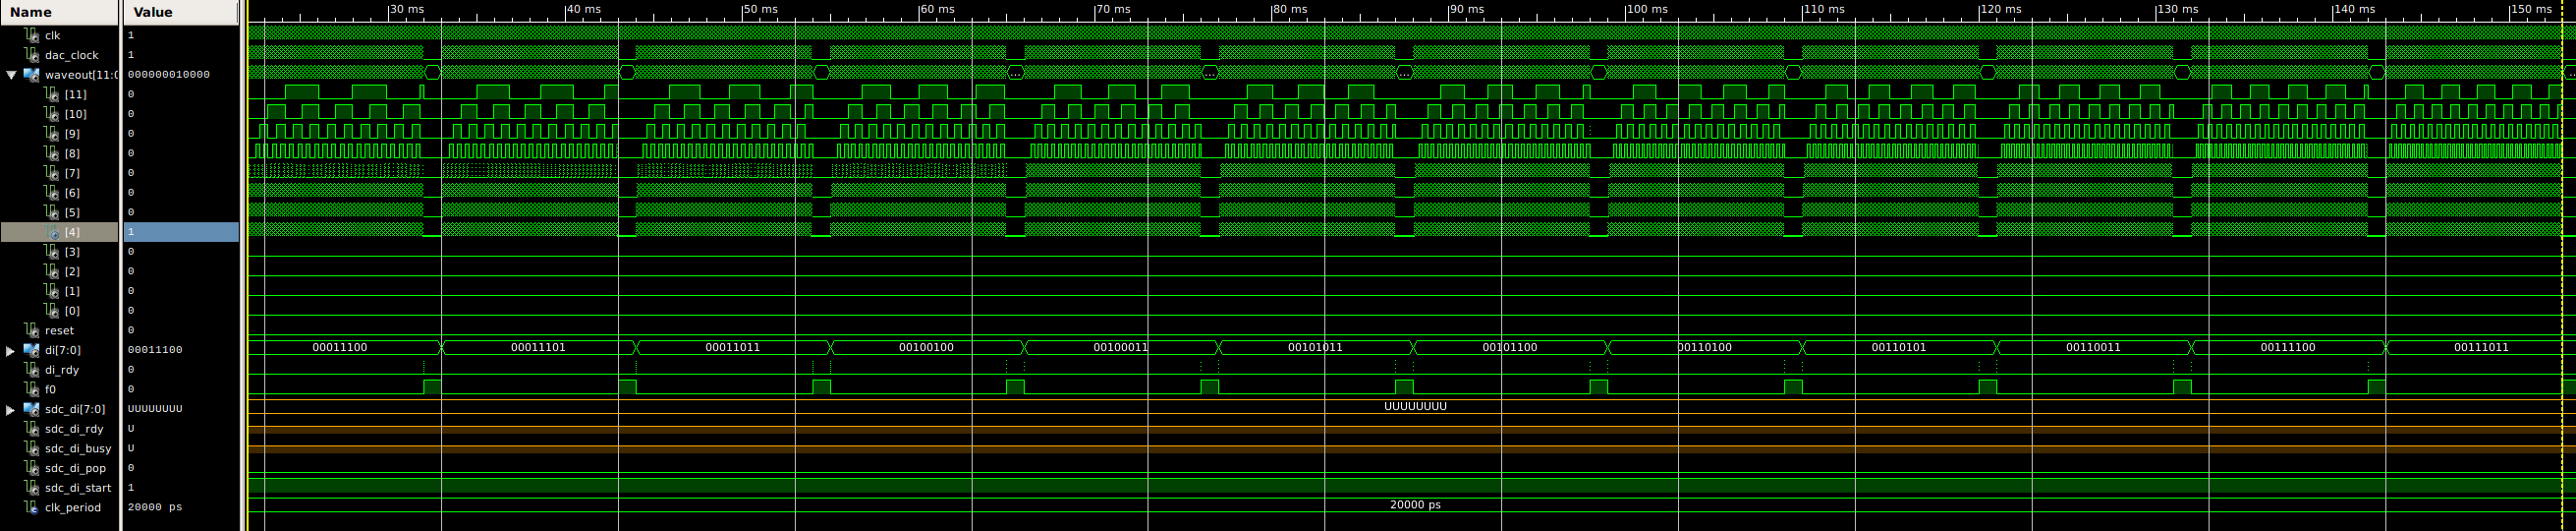
\includegraphics[decodearray={1 0 1 0 1 0}, width=\linewidth]{images/inner_sim_kb}
  \caption{Symulacja modułu InnerLogic. Wejście z klawiatury.}
  \label{sim:kb}
\end{figure}

\subsection{Wejście z karty pamięci}
Symulacja obejmuje odtworzenie melodii zdefiniowanej w pliku na karcie pamięci. Dźwięki opisane są następującym ciągiem:
\begin{lstlisting}
a403w403s403e403d403f403t403g403y403h403u403j403
\end{lstlisting}
\begin{figure}[h]
  \centering
  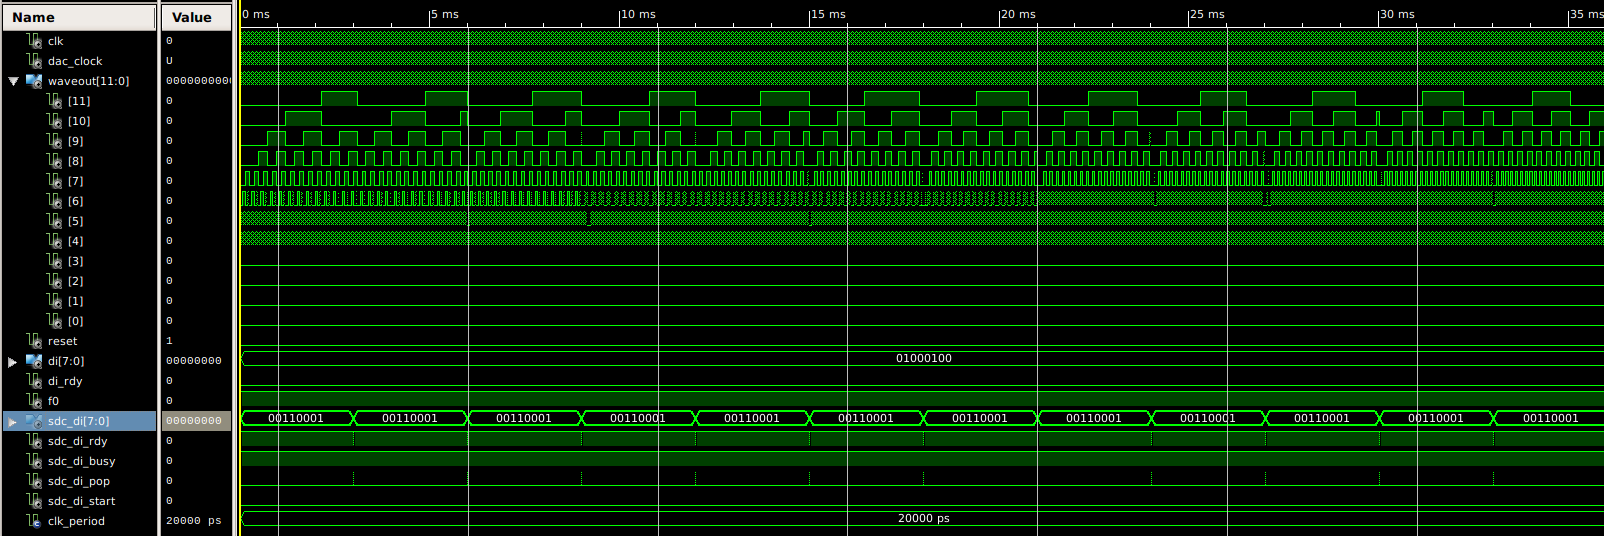
\includegraphics[decodearray={1 0 1 0 1 0}, width=\linewidth]{images/inner_sim_sd}
  \caption{Symulacja modułu InnerLogic. Wejście z karty pamięci.}
  \label{sim:sd}
\end{figure}
\clearpage

\section{Implementacja}
\subsection{Analiza czasów}
Narzędzie ISE w wygenerowanym raporcie z procesu implementacji zapewnił, że wymagania czasowe związane z częstotliwością taktowania zegara 50MHz zostaną spełnione.
\begin{lstlisting}
Timing summary: 
--------------- 
Timing errors: 0  Score: 0  (Setup/Max: 0, Hold: 0) 
Constraints cover 10400333 paths, 0 nets, and 8116 connections 
Design statistics: 
    Minimum period:  18.392ns{1}   (Maximum frequency:  54.371MHz) 
\end{lstlisting}

\subsection{Analiza zajętości zasobów}
\begin{figure}[h]
  \centering
  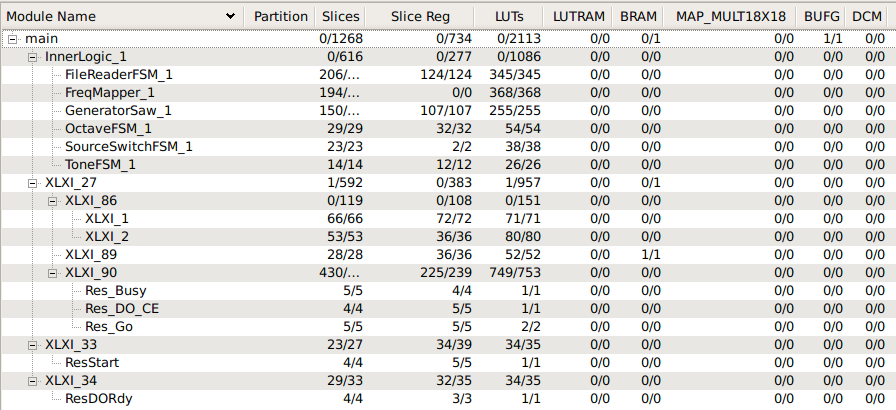
\includegraphics[width=\linewidth]{images/area}
  \caption{Raport zajętości zasobów.}
  \label{hardware}
\end{figure}

\section{Podręcznik użytkowania}

\section{Podsumowanie}

\subsection{Zrealizowane założenia}
Działanie poparte poprawnymi efektami symulacji pozwala sądzić, iż projekt został wykonany poprawnie, zgodnie ze wstępnymi założeniami. Zrezygnowano jednak z pozostałych generatorów typów fal, pozostając tylko przy fali piłokształtnej. Proces generowania fali w pozostałych generatorach odbywałby się podobnie, poprzez użycie innego zachowania liczników lub podawanie na wyjście stablicowanych wartości.

\subsection{Możliwości dalszego rozwoju}
Kolejnym etapem rozwoju projektu może być dodanie innych typów generatorów fal, oraz możliwości przełączania się pomiędzy nimi z użyciem sygnałów wejściowych, czy to z klawiatury, czy na przykład z enkodera. W następnej kolejności zrealizować można obsługę więcej niż jednego przycisku w tym samym czasie.

\clearpage
\section{Listingi}

\lstinputlisting[language=VHDL, firstline=49, lastline=101, caption={Opis architektury modułu SourceSwitchFSM}, label={lst:SourceSwitchFSM}]{../../SourceSwitchFSM.vhd}

\lstinputlisting[language=VHDL, firstline=54, lastline=67, caption={Opis architektury modułu FreqMapper}, label={lst:freqMapper}]{../../FreqMapper.vhd}


\end{document}